%% Copyright (c) 2004  SciSoft.  All rights reserved.
%%
%% This file is part of CGAL (www.cgal.org).
%% You can redistribute it and/or modify it under the terms of the GNU
%% General Public License as published by the Free Software Foundation,
%% either version 3 of the License, or (at your option) any later version.
%%
%% Licensees holding a valid commercial license may use this file in
%% accordance with the commercial license agreement provided with the software.
%%
%% This file is provided AS IS with NO WARRANTY OF ANY KIND, INCLUDING THE
%% WARRANTY OF DESIGN, MERCHANTABILITY AND FITNESS FOR A PARTICULAR PURPOSE.
%%
%% 
%%
%% Author(s)     : Fernando Cacciola <fernando_cacciola@hotmail.com>

\section{Definitions}

\subsection{2D Contour}

A {\em 2D contour} is a closed sequence (a cycle) of 3 or more \textit{connected 2D oriented straight line segments} called {\em contour edges}. The endpoints of the contour edges are called {\em vertices}. Each contour edge shares its endpoints with at least two other contour edges.\\
If the edges intersect only at the vertices and at most are coincident along a line but do not {\em cross} one another, the contour is classified as {\em simple}.\\
A contour is topologically equivalent to a \textit{disk} and if it is simple, is said to be a \textit{Jordan Curve}.\\
Contours partition the plane in two open regions: one bounded and one unbounded. If the bounded region of a contour is only one \textit{singly-connected set}, the contour is said to be {\em strictly-simple}.\\
The \ccc{Orientation} of a contour is given by the order of the vertices around the region they bound. It can be \ccc{CLOCKWISE} (CCW) or \ccc{COUNTERCLOCKWISE} (CW).\\
The {\em bounded side} of a contour edge is the side facing the bounded region of the contour. If the contour is oriented CCW, the bounded side of an edge is its left side.

A contour with a null edge (a segment of length zero given by two consecutive coincident vertices), or with edges not connected to the bounded region (an antenna: 2 consecutive edges going forth and back along the same line), is said to be {\em degenerate} (collinear edges are \textit{not} considered a degeneracy).

\subsection{2D Polygon with Holes}

A {\em 2D polygon} is a contour.\\
A {\em 2D polygon with holes} is a contour, called the {\em outer contour}, having zero or more contours, called {\em inner contours}, or {\em holes}, in its bounded region. The intersection of the bounded region of the outer contour and the unbounded regions of each inner contour is the {\em interior} of the polygon with holes. The orientation of the holes must be opposite to the orientation of the outer contour and there cannot be any intersection among any contour. A hole cannot be in the bounded region of any other hole.\\
A polygon with holes is strictly-simple if its interior is a singly-connected set.\\
The orientation of a polygon with holes is the orientation of its outer contour. The bounded side of \textit{any} edge, whether of the outer contour or a hole, is the \textit{same} for all edges. That is, if the outer contour is oriented CCW and the holes CW, both contour and hole edges face the polygon interior to their left.\\

Throughout the rest of this chapter the term {\em polygon} will be used as a shortcut for {\em polygon with holes}. 

\begin{figure}[htbp]
\begin{ccTexOnly}
\begin{center}
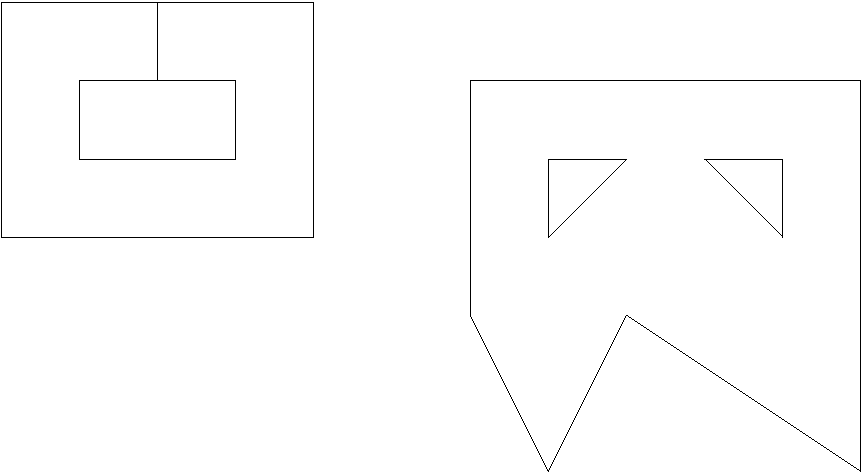
\includegraphics{Straight_skeleton_2/valid_polygons} % omit suffix .eps to support PS and PDF
\end{center}
\end{ccTexOnly}
\begin{ccHtmlOnly}
<TABLE CELLSPACING=40>
<TR>
<CENTER>
<IMG BORDER=0 SRC="./valid_polygons.png" ALIGN=middle ALT="Valid polygons">
</CENTER>
</TR>
</TABLE>
\end{ccHtmlOnly}
\caption{Examples of strictly simple polygons: One with no holes and two edges coincident (left) and one with 2 holes (right).
\label{Valid-polygons}}
\end{figure}

\begin{figure}[htbp]
\begin{ccTexOnly}
\begin{center}
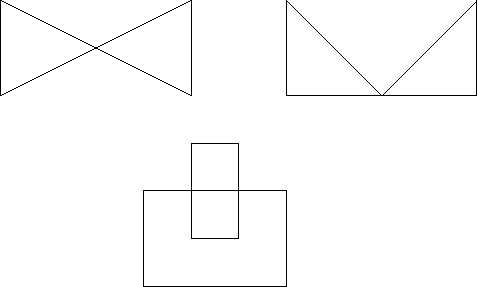
\includegraphics{Straight_skeleton_2/invalid_polygons} % omit suffix .eps to support PS and PDF
\end{center}
\end{ccTexOnly}
\begin{ccHtmlOnly}
<TABLE CELLSPACING=40>
<TR>
<CENTER>
<IMG BORDER=0 SRC="./invalid_polygons.png" ALIGN=middle ALT="Valid polygons">
</CENTER>
</TR>
</TABLE>
\end{ccHtmlOnly}
\caption{Examples of non-simple polygons: One folding into itself, that is, non-planar (left), one with a vertex touching an edge (right), and one with a hole crossing into the outside (bottom)
\label{Invalid-polygons}}
\end{figure}

\subsection{Inward Offset of a Non-degenerate Strictly-Simple Polygon with Holes}

For any 2D non-degenerate strictly-simple polygon with holes called the {\em source}, there can exist a \textit{set} of 0, 1 or more {\em inward offset polygons with holes}, or just offset polygons for short, at some euclidean distance \textit{t} $>0$ (each being strictly simple and non-degenerate). Any contour edge of such offset polygon, called an {\em offset edge} corresponds to \textit{some} contour edge of the source polygon, called its {\em source edge}. An offset edge is parallel to its source edge and has the same orientation. The Euclidean distance between the \textit{lines} supporting an offset edge and its source edge is exactly \ccc{t}.\\
An offset edge is always located to the bounded side of its source edge (which is an oriented straight line segment).\\
An offset polygon can have less, equal or more sides as its source polygon.\\
If the source polygon has no holes, no offset polygon has holes. If the source polygon has holes, any of the offset polygons can have holes itself, but it might as well have no holes at all (if the distance is sufficiently large).\\
Each offset polygon has the same orientation as the source polygon.

\begin{figure}[htbp]
\begin{ccTexOnly}
\begin{center}
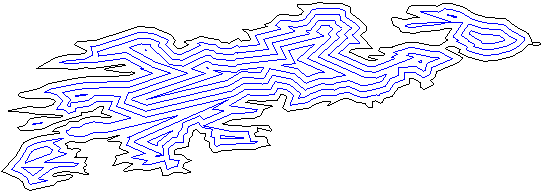
\includegraphics{Straight_skeleton_2/complex_offset} % omit suffix .eps to support PS and PDF
\end{center}
\end{ccTexOnly}
\begin{ccHtmlOnly}
<TABLE CELLSPACING=40>
<TR>
<CENTER>
<IMG BORDER=0 SRC="./complex_offset.png" ALIGN=middle ALT="Offset contours of a shaggy polygon">
</CENTER>
</TR>
</TABLE>
\end{ccHtmlOnly}
\caption{Offset contours of a sample polygon
\label{Offsets}}
\end{figure}

\subsection{Straight Skeleton of a 2D Non-degenerate Strictly-Simple Polygon with Holes}
 
The {\em 2D straight skeleton} of a non-degenerate strictly-simple polygon with holes \cite{aaag-ntsp-95} is a special partitioning of the polygon interior into {\em straight skeleton regions} corresponding to the monotone areas traced by a continuous \textit{inward offsetting} of the contour edges. Each region corresponds to exactly 1 contour edge.\\
These regions are bounded by angular bisectors of the supporting lines of the contour edges and each such region is itself a non-convex non-degenerate strictly-simple polygon.

\begin{figure}[htbp]
\begin{ccTexOnly}
\begin{center}
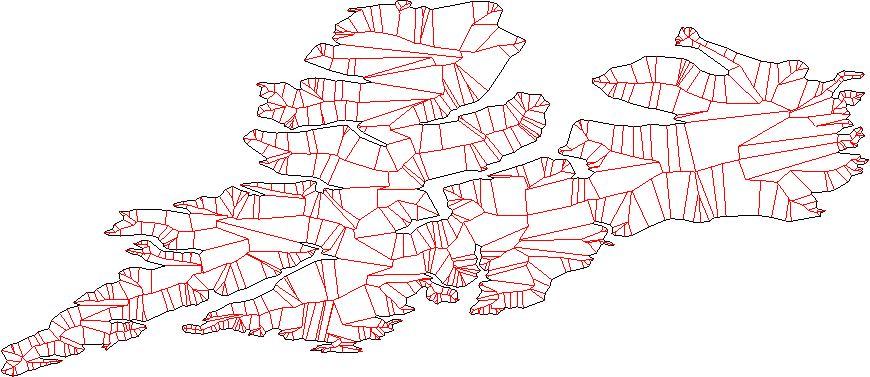
\includegraphics{Straight_skeleton_2/complex_skeleton} % omit suffix .eps to support PS and PDF
\end{center}
\end{ccTexOnly}

\begin{ccHtmlOnly}
<TABLE CELLSPACING=40>
<TR>
<CENTER>
<IMG BORDER=0 SRC="./complex_skeleton.png" ALIGN=middle ALT="Complex Straight Skeleton">
</CENTER>
</TR>
</TABLE>
\end{ccHtmlOnly}

\caption{Straight skeleton of a complex shaggy contour
\label{ComplexSLS}}
\end{figure}

\begin{figure}[htbp]
\begin{ccTexOnly}
\begin{center}
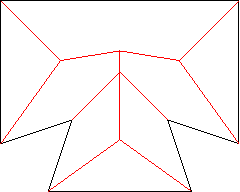
\includegraphics{Straight_skeleton_2/simple_skeleton_0} % omit suffix .eps to support PS and PDF
\end{center}
\begin{center}
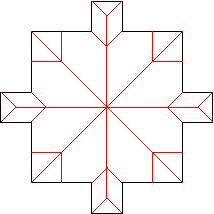
\includegraphics{Straight_skeleton_2/simple_skeleton_1} % omit suffix .eps to support PS and PDF
\end{center}
\begin{center}
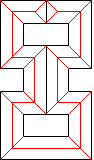
\includegraphics{Straight_skeleton_2/validly_touching} % omit suffix .eps to support PS and PDF
\end{center}
\end{ccTexOnly}

\begin{ccHtmlOnly}
<TABLE CELLSPACING=40>
<TR>
<CENTER>
<TD>
<CENTER>
<IMG BORDER=0 SRC="./simple_skeleton_0.png" ALIGN=middle ALT="Complex Straight Skeleton">
</CENTER>
</TD>
<TD>
<CENTER>
<IMG BORDER=0 SRC="./simple_skeleton_1.png" ALIGN=middle ALT="Complex Straight Skeleton">
</CENTER>
</TD>
<TD>
<CENTER>
<IMG BORDER=0 SRC="./validly_touching.png" ALIGN=middle ALT="A validly touching polygon">
</CENTER>
</TD>
</CENTER>
</TR>
</TABLE>
\end{ccHtmlOnly}

\caption{Other examples: A vertex-event (left), the case of several collinear edges (middle), and the case of a validly simple polygon with tangent edges (right).
\label{MoreSLS}}
\end{figure}
  
\subsubsection{Angular Bisecting Lines and Offset Bisectors}  

Given two points and a line passing through them, the perpendicular line passing through the midpoint is the bisecting line (or bisector) of those points.

Two non-parallel lines, intersecting at a point, are bisected by two
other lines passing through that intersection point.

Two parallel lines are bisected by another parallel line placed
halfway in between.

Given just one line, any perpendicular line can be considered the
bisecting line (any bisector of any two points along the single line).

The bisecting lines of two edges are the lines bisecting the
supporting lines of the edges (if the edges are parallel or collinear,
there is just one bisecting line).

The halfplane to the bounded side of the line supporting a contour edge is
called the {\em offset zone} of the contour edge.

Given any number of contour edges (not necessarily consecutive), the
intersection of their offset zones is called their {\em combined
offset zone}.

Any two contour edges define an {\em offset bisector}, as follows: If
the edges are non-parallel, their bisecting lines can be decomposed as
4 rays originating at the intersection of the supporting lines. Only
one of these rays is contained in the combined offset zone of the
edges (which one depends on the possible combinations of
orientations). This ray is the offset bisector of the non-parallel
contour edges.

If the edges are parallel (but not collinear) and have opposite
orientation, the entire and unique bisecting line is their offset
bisector. If the edges are parallel but have the same orientation,
there is no offset bisector between them.

If the edges are collinear and have the same orientation, their offset
bisector is given by a perpendicular ray to the left of the edges
which originates at the midpoint of the combined complement of
the edges. (The {\em complement} of an edge/segment are the two
rays along its supporting line which are not the segment and the
{\em combined complement} of \ccc{N} collinear segments is the
intersection of the complements of each segment). If the edges are
collinear but have opposite orientation, there is no offset bisector
between them.

%% Figure of bisecting lines and offset bisectors here

\subsubsection{Faces, Edges and Vertices}

Each region of the partitioning defined by a straight skeleton is
called a {\em face}. Each face is bounded by straight line segments,
called {\em edges}. Exactly one edge per face is a {\em contour edge}
(corresponds to a side of the polygon) and the rest of the edges,
located in the interior of the polygon, are called {\em skeleton
edges}, or {\em bisectors}.

The bisectors of the straight skeleton are segments of the offset
bisectors as defined previously. Since an offset bisector is a ray of
a bisecting line of 2 contour edges, each skeleton edge (or bisector)
is uniquely given by two contour edges. These edges are called the
{\em defining contour edges} of the bisector.

The intersection of the edges are called {\em vertices}. Although in a
simple polygon, only 2 edges intersect at a vertex, in a straight
skeleton, 3 or more edges intersect a any given vertex. That is, vertices in a
straight skeleton have degree $>=3$.

A {\em contour vertex} is a vertex for which 2 of its incident edges are contour edges.

A {\em skeleton vertex} is a vertex who's incident edges are all skeleton edges.

A {\em contour bisector} is a bisector who's defining contour edges
are consecutive. Such a bisector is incident upon 1 contour vertex and
1 skeleton vertex and touches the input polygon at exactly 1 endpoint.

An {\em inner bisector} is a bisector who's defining contour edges are
not consecutive. Such a bisector is incident upon 2 skeleton vertices
and is strictly contained in the interior of the polygon.

\section{Representation}

This \cgal\ package represents a straight skeleton as a specialized \ccc{Halfedge Data Structure} (HDS) whose vertices embeds 2D Points (see the \ccc{StraightSkeleton_2} concept in the reference manual for details).

Its halfedges, by considering the source and target points, implicitly embeds 2D oriented straight line segments (each halfedge per see does not embed a segment explicitly).

A face of the straight skeleton is represented as a face in the
HDS. Both contour and skeleton edges are represented by pairs of
opposite HDS halfedges, and both contour and skeleton vertices are
represented by HDS vertices.

In a HDS, a border halfedge is a halfedge which is incident upon an
unbounded face. In the case of the straight skeleton HDS, such border
halfedges are oriented such that their left side faces outwards the
polygon. Therefore, the opposite halfedge of any border halfedge is
oriented such that its left side faces inward the polygon.

This \cgal\ package requires the input polygon (with holes) to be non-degenerate,
strictly-simple, and oriented counter-clockwise.

The skeleton halfedges are oriented such that their \textit{left} side faces
inward the region they bound. That is, the vertices (both contour and
skeleton) of a face are circulated in counter-clockwise order. There
is one and only one contour halfedge incident upon any face.

The contours of the input polygon are traced by the border halfedges 
of the HDS (those facing outward), but in the opposite direction. That 
is, the vertices of the contours can only by traced from the straight
skeleton data structure by circulating the border halfedges,
and the resulting vertex sequence will be reversed w.r.t 
the input vertex sequence.

A skeleton edge, according to the definition given in the previous
section, is defined by 2 contour edges. In the representation, each
one of the opposite halfedges that represent a skeleton edge is
associated with one of the opposite halfedges that correspond to one
of its defining contour edges. Thus, the 2 opposite halfedges of a
skeleton edge link the edge to its 2 defining contour edges.

Starting from any border contour halfedge, circulating the structure
walks through border counter halfedges and traces the vertices of the
polygon's contours (in opposite order).

Starting from any non-border but contour halfedge, circulating the
structure walks counter-clockwise around the face corresponding
to that contour halfedge. The vertices around a face always describe
a non-convex non-degenerate strictly-simple polygon.

A vertex is the intersection of contour and/or skeleton edges. Since a
skeleton edge is defined by 2 contour edges, any vertex is itself
defined by a unique set of contour edges. These are called the
{\em defining contour edges} of the vertex.

A vertex is identified by it's set of defining contour edges. Two
vertices are distinct if they have differing sets of defining contour
edges.  Note that vertices can be distinct even if they are geometrically
embedded at the same point.

The {\em degree} of a vertex is the number of halfedges around the vertex 
incident upon (pointing to) the vertex. As with any halfedge data structure,
there is one outgoing halfedge for each incoming (incident) halfedge around
a vertex. The degree of the vertex counts only incoming (incident) halfedges.

In a straight skeleton, the degree of a vertex is not only the number of
incident halfedges around the vertex but also the number of defining contour
halfedges. The vertex itself is the point where all the defining
contour edges simultaneously collide.

Contour vertices have exactly two defining contour halfedges, which are
the contour edges incident upon the vertex; and 3 incident halfedges.
One and only one of the incident halfedges is a skeleton halfedge.
The degree of a contour vertex is exactly 3.

Skeleton vertices have at least 3 defining contour halfedges and 3 incident skeleton halfedges.
If more than 3 edges collide simultaneously at the same point and time (like in any regular polygon
with more than 3 sides), the corresponding skeleton vertex will have more than 3 defining contour
halfedges and incident skeleton halfedges. That is, the degree of a skeleton vertex is $>=3$ 
(the algorithm initially produces nodes of degree 3 but in the end all coincident nodes are merged to form higher degree nodes). All halfedges incident upon a skeleton vertex are skeleton halfedges.

The defining contour halfedges and incident halfedges around a vertex can be traced using the circulators provided by the vertex class. The degree of a vertex is not cached and cannot be directly obtained from the vertex, but you can calculate this number by manually counting the number of incident halfedges around the vertex.

Each vertex stores a 2D point and a \ccc{time}, which is the euclidean distance from the vertex's point to the \textit{lines} supporting each of the defining contour edges of the vertex (the distance is the same to each line). Unless the polygon is convex, this distance is not equidistant to the edges, as in the case of a Medial Axis, therefore, the time of a skeleton vertex does not correspond to the distance from the polygon to the vertex (so it cannot be used to obtain the deep of a region in a shape, for instance).\\
If the polygon \textit{is} convex, the straight skeleton is exactly equivalent to the polygon's Voronoi diagram and each vertex time is the equidistance to the defining edges.\\
Contour vertices have time zero.

\begin{figure}[htbp]
\begin{ccTexOnly}
\begin{center}
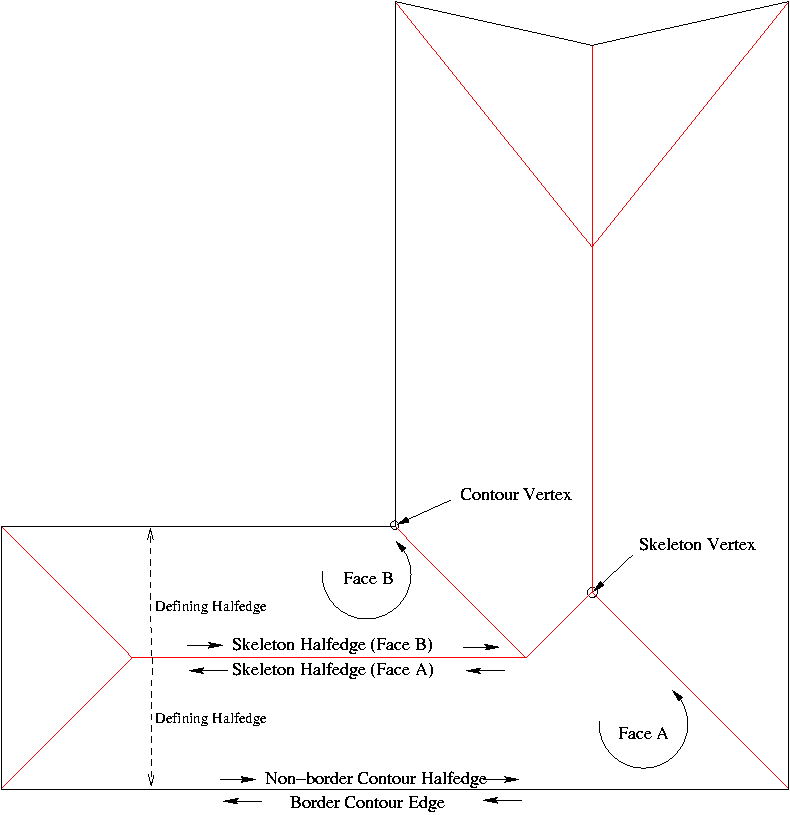
\includegraphics{Straight_skeleton_2/fig6} % omit suffix .eps to support PS and PDF
\end{center}
\end{ccTexOnly}

\begin{ccHtmlOnly}
<TABLE CELLSPACING=40>
<TR>
<TD>
<CENTER>
<IMG BORDER=0 SRC="./fig6.png" ALIGN=middle ALT="Straight skeleton DS">
</CENTER>
</TD>
</TR>
</TABLE>
\end{ccHtmlOnly}

\caption{Straight Skeleton Data Structure
\label{Simplepoly-offsets}}
\end{figure}

\section{API}

\subsection{Create a Straight Skeleton}

The straight skeleton data structure is defined by the \ccc{StraightSkeleton_2} concept and modeled in the \ccc{Straight_skeleton_2<Traits,Items,Alloc>} class.

The simplest way to construct a straight skeleton is via the free functions \ccc{create_interior_straight_skeleton_2} and \ccc{create_exterior_straight_skeleton_2}, as shown in the following example:

\ccIncludeExampleCode{Straight_skeleton_2/Create_straight_skeleton_2.cpp}

The input to these functions is the polygon, which can be given as an iterator pair or directly as a \ccc{Polygon_2} object. In the case of the exterior skeleton, a maximum offset must be specified as well (see the ref manual for details on this max offset parameter).

\subsection{Create a Straight Skeleton from a Polygon With Holes}

If \ccc{Polygon_with_holes_2} is used, you can pass an instance of it directly to the function creating the interior skeleton, as shown below. Notice that a different header must be included in this case. 

\ccIncludeExampleCode{Straight_skeleton_2/Create_straight_skeleton_from_polygon_with_holes_2.cpp}

\subsection{Create Offset Polygons from a Straight Skeleton}

If you already have a straight skeleton instance, the simpler way to generate offset polygons is to call \ccc{create_offset_polygons_2} as shown in the next example, passing the desired offset and the straight skeleton. You can reuse the same skeleton to generate offsets at a different distance, which is recommended because producing the straight skeleton is much slower then generating offset polygons.

\ccIncludeExampleCode{Straight_skeleton_2/Create_offset_polygons_2.cpp}

\subsection{Create Offset Polygons from a Polygon (With or Without Holes)}

If you need offset polygons at just one single distance, you can hide away the construction of the straight skeleton by calling directly the functions \ccc{create_interior_skeleton_and_offset_polygons_2} and \ccc{create_exterior_skeleton_and_offset_polygons_2} as shown in the following examples:

\ccIncludeExampleCode{Straight_skeleton_2/Create_skeleton_and_offset_polygons_2.cpp}

... and using a \ccc{Polygon_with_holes_2} directly when available:

\ccIncludeExampleCode{Straight_skeleton_2/Create_saop_from_polygon_with_holes_2.cpp}

If the input polygon has holes, there can be holes in the offset polygons. 
However, the polygons generated by all the offsetting functions shown before
do not have any parent-hole relationship computed; that is, they just instances
of \ccc{Polygon_2} instead of \ccc{Polygon_with_holes_2}. 
If \ccc{Polygon_with_holes_2} are available and you need the offsetting to produce them, you can call the function \ccc{arrange_offset_polygons_2} passing the result of any of the offsetting functions described so far. That function arranges the offset polygons detecting and distributing holes within parents.
As a shortcut, you can use the function \ccc{create_interior_skeleton_and_offset_polygon_with_holes_2} as shown below:

\ccIncludeExampleCode{Straight_skeleton_2/Create_skeleton_and_offset_polygons_with_holes_2.cpp}

\begin{ccAdvanced}
Consider an input polygon with parallel edges separated a distance $2*t$. If you produce an offset polygon at distance $t$, these parallel edges  will just collapse each other and vanish from the result, keeping the output as a {\em simple polygon}, just like the input. However, if you request an offset polygon at a distance $t-epsilon$, the result will still be a simple polygon but with edges that are so close to each other that will almost intersect. 
If a kernel with exact constructions is used, the offsetting algorithm can guarantee that the output contains only simple polygons. However, if inexact constructions are used the roundoff in the coordinates of the output points will cause parallel edges that {\em almost} collapse-but not so-to become really collinear or even cross each other. 

Thus, it is neccessary to use a kernel with exact constructions if offset polygons must be simple, yet computing a straight skeleton using that kernel is very slow, much more than computing the offset polygons. To help with this, it is possible to construct the straight skeleton using the recommended kernel \ccc{Exact_predicates_inexact_constructions_kernel}, then convert the skeleton to a different kernel via the function \ccc{convert_straight_skeleton_2} and input the converted skeleton to the offsetting functions.

All the offsetting functions that take polygons as input (and create the straight skeleton under the hood) apply that optimization automatically: that is, the output polygons are defined over the same kernel of the input polygons, whatever that is, yet the straight skeleton is constructed with the faster recommended kernel and converted if necessary.

Notice how some of the examples above use \ccc{Exact_predicates_exact_constructions_kernel}. In all cases, the straight skeleton is constructed using \ccc{Exact_predicates_inexact_constructions_kernel}.

\end{ccAdvanced}

\subsection{Low level API}

All the high level functions described above are just wrappers around the low level 
API described here. This low level API is richer and provides options and configurations 
not covered by any of those functions.

The straight skeleton construction algorithm is encapsulated in the
class \ccc{Straight_skeleton_builder_2<Gt,Ss,Visitor>} which is
parameterized on a geometric traits (class
\ccc{Straight_skeleton_builder_traits<Kernel>}) and the Straight
Skeleton class (Ss).

The offset contours construction algorithm is encapsulated in the class
\ccc{Polygon_offset_builder_2<Ss,Gt,Container>} which is
parameterized on the Straight Skeleton class (Ss), a
geometric traits (class \ccc{Polygon_offset_builder_traits<Kernel>})
and a container type where the resulting offset polygons are
generated.

To construct the straight skeleton of a polygon with holes the user must:
 
(1) Instantiate the straight skeleton builder.

(2) Enter one contour at a time, starting from the outer contour, via
    the method \ccc{enter_contour}. The input polygon with holes must be 
    non-degenerate, strictly-simple and counter-clockwise oriented
    (see the definitions at the beginning of this chapter).
    Collinear edges are allowed. The insertion order of each hole
    is unimportant but the outer contour must be entered first.

(3) Call \ccc{construct_skeleton} once \textit{all} the contours have been entered. You
cannot enter another contour once the skeleton has been constructed.

To construct a set of inward offset contours the user must:
 
(1) Construct the straight skeleton of the source polygon with holes.

(2) Instantiate the polygon offset builder passing in the straight skeleton as a parameter.

(3) Call \ccc{construct_offset_contours} passing the desired offset
    distance and an output iterator that can store a
    \ccc{boost::shared_ptr} of \ccc{Container} instances 
    into a resulting sequence (typically, a back insertion iterator)
    
Each element in the resulting sequence is an {\em offset contour}, given by
a \ccc{boost::shared_ptr} holding a dynamically allocated instance 
of the Container type. Such a container can be any model of the 
\ccc{VertexContainer_2} concept, for example, a \ccc{CGAL::Polygon_2}, 
or just a \ccc{std::vector} of 2D points.

The resulting sequence of offset contours can contain both outer and inner contours. 
Each offset hole (inner offset contour) would logically belong in the interior of some 
of the outer offset contours.
However, this algorithm returns a sequence of contours in arbitrary order and there is no
indication whatsoever of the parental relationship between inner and outer contours.

On the other hand, each outer contour is counter-clockwise oriented while each hole is clockwise-oriented.
And since offset contours do form simple polygons with holes, it is guaranteed that no hole will be inside another hole, no outer contour will be inside any other contour, and each hole will be inside exactly 1 outer contour.

Parental relationships are {\em not} automatically reconstructed by this algorithm because this relation is not directly given by the input polygon with holes and must be done as a post processing step. The function \ccc{arrange_offset_polygons_2} can be used to do that efficiently.

A user can reconstruct the parental relationships as a post processing operation 
by testing each inner contour (which is identified by being clockwise) against each outer contour (identified as being counter-clockwise) for insideness.

This algorithm requires exact predicates but not exact constructions
Therefore, the \ccc{Exact_predicates_inexact_constructions_kernel} should be used.

\ccIncludeExampleCode{Straight_skeleton_2/Low_level_API.cpp}

\subsection{Exterior Skeletons and Exterior Offset contours}  

This \cgal\ package can only construct the straight skeleton and offset contours in the \textit{interior} of a polygon with holes. However, constructing exterior skeletons and exterior offsets is possible:

Say you have some polygon made of 1 outer contour C0 and 1 hole C1, and you need to obtain some exterior offset contours.\\
The interior region of a polygon with holes is connected while the exterior region is not: there is an unbounded region outside the outer contour, and one bounded region inside each hole.
To construct an offset contour you need to construct an straight skeleton. Thus, to construct exterior offset contours for a polygon with holes, you need to construct, {\em separately}, the exterior skeleton of the outer contour and the interior skeleton of each hole.\\
Constructing the interior skeleton of a hole is directly supported by this \cgal\ package; you just need to input the hole's vertices in reversed order as if it were an outer contour.\\
Constructing the exterior skeleton of the outer contour is possible by means of the following trick: place the contour as a hole of a big rectangle (call it {\em frame}). If the frame is sufficiently separated from the contour, the resulting skeleton will be practically equivalent to a \textit{real} exterior skeleton.\\
To construct exterior offset contours in the inside of each hole you just use the skeleton constructed in the interior, and, if required, revert the orientation of each resulting offset contour.\\
Constructing exterior offset contours in the outside of the outer contour is just a little bit more involved: Since the contour is placed as a hole of a frame, you will always obtain 2 offset contours for any given distance; one is the offseted frame and the other is the offseted contour. Thus, from the resulting offset contour sequence, you always need to discard the offsetted frame, easily identified as the offset contour with the largest area.\\
It is necessary to place the frame sufficiently away from the contour. If it is not, it could occur that the outward offset contour collides and merges with the inward offset frame, resulting in 1 instead of 2 offset contours.\\
However, the proper separation between the contour and the frame is not directly given by the offset distance at which you want the offset contour. That distance must be at least the desired offset plus the largest euclidean distance between an offset vertex and its original.\\
This \cgal\ packages provides a helper function to compute the required separation:
\ccc{compute_outer_frame_margin}\\
If you use this function to place the outer frame you are guaranteed to obtain an offset contour corresponding exclusively to the frame, which you can always identify as the one with the largest area and which you can simple remove from the result (to keep just the relevant outer contours).

\begin{figure}[htbp]
\begin{ccTexOnly}
\begin{center}
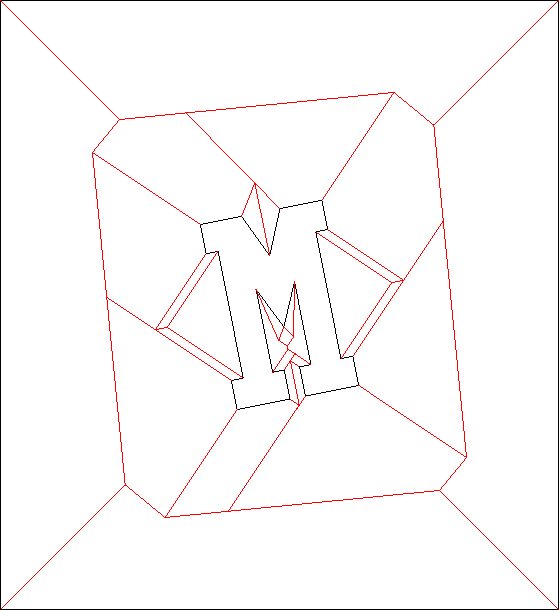
\includegraphics{Straight_skeleton_2/exterior_skeleton} % omit suffix .eps to support PS and PDF
\end{center}
\begin{center}
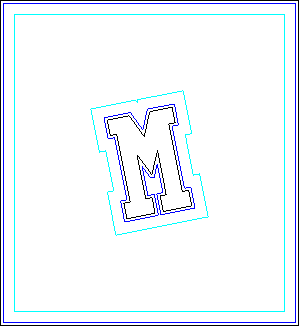
\includegraphics{Straight_skeleton_2/exterior_offset} % omit suffix .eps to support PS and PDF
\end{center}
\end{ccTexOnly}

\begin{ccHtmlOnly}
<TABLE CELLSPACING=40>
<TR>
<TD>
<CENTER>
<IMG BORDER=0 SRC="./exterior_skeleton.png" ALIGN=middle ALT="Complex Straight Skeleton">
</CENTER>
</TD>
<TD>
<CENTER>
<IMG BORDER=0 SRC="./exterior_offset.png" ALIGN=middle ALT="Complex Straight Skeleton">
</CENTER>
</TD>
</TR>
</TABLE>
\end{ccHtmlOnly}

\caption{Exterior skeleton obtained using a frame (left) and 2 sample exterior offset contours (right)
\label{Exterior}}
\end{figure}


\section{Straight Skeletons, Medial Axis and Voronoi Diagrams}  

The straight skeleton of a polygon is similar to the medial
axis and the Voronoi diagram of a polygon in the way it partitions
it; however, unlike the medial axis and Voronoi diagram, the
bisectors are not equidistant to its defining edges but to the
supporting lines of such edges. As a result, Straight Skeleton
bisectors might not be located in the center of the polygon and so
cannot be regarded as a proper Medial Axis in its geometrical meaning.

On the other hand, only reflex vertices (whose internal angle $>pi$)
are the source of deviations of the bisectors from its center
location. Therefore, for convex polygons, the straight skeleton, the
medial axis and the Voronoi diagram are exactly equivalent,
and, if a non-convex polygon contains only vertices of low
reflexivity, the straight skeleton bisectors will be placed nearly
equidistant to their defining edges, producing a straight skeleton
pretty much alike a proper medial axis.

%% Straight Skeleton, Medial Axis and Voronoi Diagram figures here

\section{Usages of the Straight Skeletons}  

The most natural usage of straight skeletons is offsetting: growing and shrinking polygons (provided by this  \cgal\ package).

Another usage, perhaps its very first, is roof design: The straight skeleton of a polygonal roof directly gives the layout of each tent. If each skeleton edge is lifted from the plane a height equal to its offset distance, the resulting roof is "correct" in that water will always fall down to the contour edges (roof border) regardless of were in the roof it falls. \cite{cgal:ld-agrm-03} gives an algorithm for roof design based on the straight skeleton.

Just like medial axes, 2D straight skeletons can also be used for 2D shape description and matching. Essentially, all the applications of image-based skeletonization (for which there is a vast literature) are also direct applications of the straight skeleton, specially since skeleton edges are simply straight line segments.

Consider the subgraph formed only by \textit{inner bisectors} (that is, only the skeleton halfedges which are not incident upon a contour vertex). Call this subgraph a {\em skeleton axis}.
Each node in the skeleton axis whose degree is $>=3$ roots more than one skeleton tree. Each skeleton tree roughly corresponds to a region in the input topologically equivalent to a rectangle; that is, without branches. For example, a simple letter "H" would contain 2 higher degree nodes separating the skeleton axis in 5 trees; while the letter "@" would contain just 1 higher degree node separating the skeleton axis in 2 curly trees. 

Since a skeleton edge is a 2D straight line, each branch in a skeleton tree is a polyline. Thus, the path-length of the tree can be directly computed. Furthermore, the polyline for a particular tree can be interpolated to obtain curve-related information.

Pruning each skeleton tree cutting off branches whose length is below some threshold; or smoothing a given branch, can be used to reconstruct the polygon without undesired details, or fit into a particular canonical shape.

Each skeleton edge in a skeleton branch is associated with 2 contour edges which are facing each other. If the polygon has a bottleneck (it almost touches itself), a search in the skeleton graph measuring the distance between each pair of contour edges will reveal the location of the bottleneck, allowing you to cut the shape in two. Likewise, if two shapes are too close to each other along some part of their boundaries (a near contact zone), a similar search in an exterior skeleton of the two shapes at once would reveal the parts of near contact, allowing you to stitch the shapes. These \textit{cut and stitch} operations can be directly executed in the straight skeleton itself instead of the input polygon (because the straight skeleton contains a graph of the connected contour edges).


\section{Straight Skeleton of a General Figure in the Plane}

A straight skeleton can also be defined for a general
multiply-connected planar directed straight-line graph \cite{aa-skfgpf-95} by considering
all the edges as embedded in an unbounded region. The only difference
is that in this case some faces will be only partially bounded.


The current version of this \cgal\ package can only construct the
straight skeleton in the interior of a simple polygon with holes, that is it
doesn't handle general polygonal figures in the plane.

% +------------------------------------------------------------------------+
%%RefPage: end of main body, begin of sfsooter
% EOF
% +------------------------------------------------------------------------+

